% src/slides/source/final/core/05_evaluation.tex

\begin{frame}{Evaluation Method}
  \SlideBody{\begin{VisualCanvas}
    \node[final heading] at (2.25,5.15) {V2X-Sim};
    \node[inner sep=0pt] at (2.25,3.5)
      {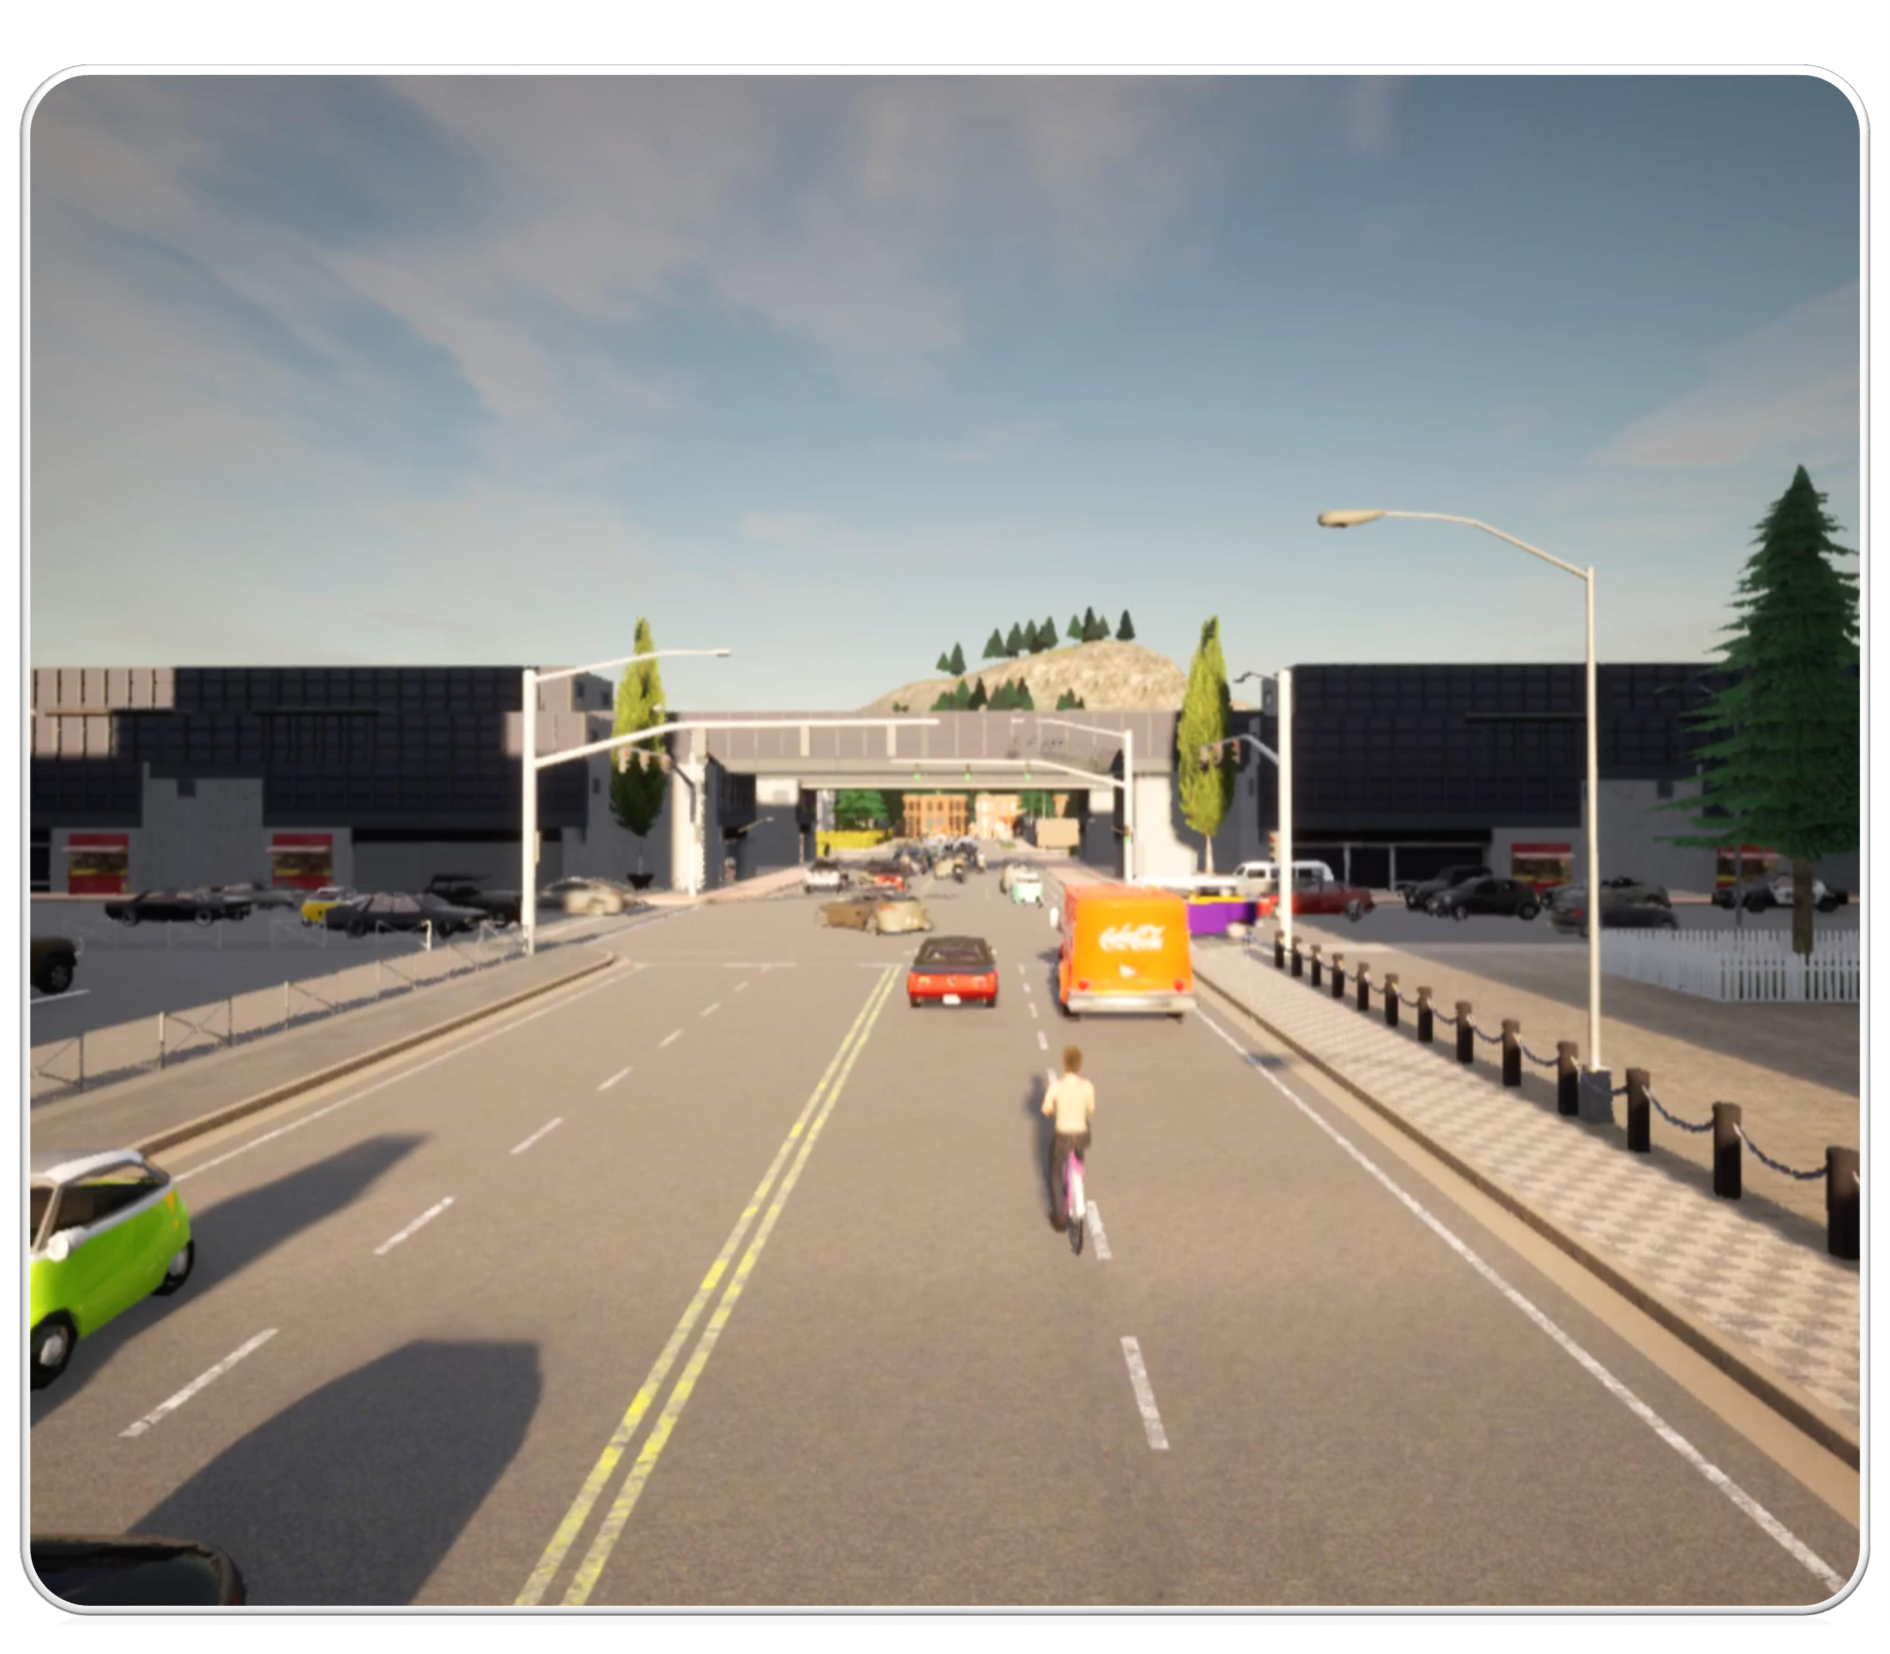
\includegraphics[width=3.5cm,height=2.35cm,keepaspectratio]{assets/papers/disconet/camera.png}};
    \node[final caption] at (2.25,1.75) {Same Held-Out Scenes};
    \tikzset{comparison method/.style={visual panel,align=center,text width=3.0cm,
      minimum height=0.8cm,font=\fontsize{12}{15}\selectfont}}
    \node[comparison method] (own) at (7.2,4.65) {Own Scan Only};
    \node[comparison method] (early) at (7.2,3.25) {Early Fusion};
    \node[comparison method] (disco) at (7.2,1.85) {DiscoNet};
    \draw[visual arrow] (4.2,3.25) -- (4.8,3.25) |- (own.west);
    \draw[visual arrow] (4.8,3.25) -- (early.west);
    \draw[visual arrow] (4.8,3.25) |- (disco.west);
    \foreach \Method in {own,early,disco} {
      \draw[draw=MoverCyan,line width=1.0pt] (\Method.east) -| (9.6,3.25);
    }
    \draw[visual arrow] (9.6,3.25) -- (10.45,3.25);
    \node[final statement] at (12.5,4.15) {AP @ 0.5};
    \node[final statement] at (12.5,3.05) {AP @ 0.7};
    \node[final caption] at (12.5,1.75) {Matched Overlays};
    \VisualTakeaway{Repeat for Each Valid $n$: AP + Latency + Peak GPU Memory}
  \end{VisualCanvas}}
  \SlideSource{Source: Li et al., Fig. 3(b). AI generated illustration.}
\end{frame}
